\hspace{24pt}
In this chapter, we will introduce the method we implemented on EAGLE to reduce the reference bias.Explain in detail how we create our hypothetical sequence based on the variant and how to quickly search through FM-index to obtain those missing reads, and finally add these reads to the pileup that we eagle considers.
\section{Overview}
The red area in Figure \ref{f3-1} shows our implementation of the core workflow of reducing reference bias on EAGLE, and the whole  Figure \ref{f3-1} is our complete workflow after combining EAGLE. 
We can roughly divide our workflow into the following five parts:
\begin{enumerate}
    \item According variant in VCF files and reference genome to create our hypothetical sequence, this sequence is important because including individual differences.
    \item Then we need to convert our FASTQ format read to FASTA format to build the FM-index of read, (For brevity, hereafter we will simply call these 'read-index'
    \item Use BWA and read-index to find the read that include variant, and then check if it in already exists in the pileup. (Multiple alignment of reads to the genome)
    \item For read that does not exist in the pileup, create read's alignment information mapped against reference sequences 
    \item Add read and alignment information in the pileup, improve the eagle calculate.

\end{enumerate}

\begin{figure}[H]
    \centering
    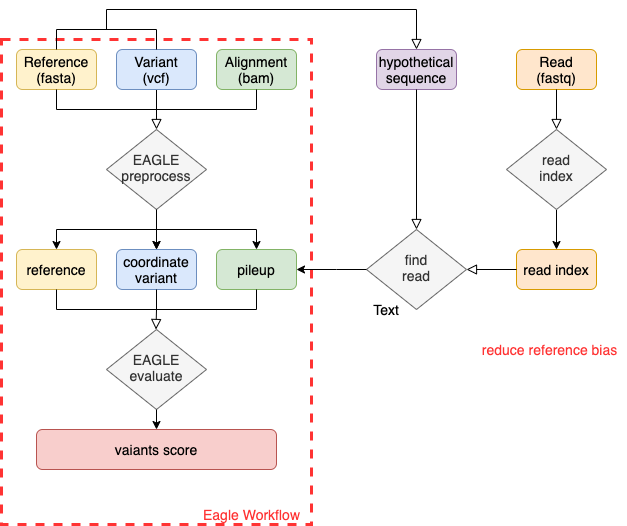
\includegraphics[width=0.8\columnwidth]{body/image/3-1.png}
    \captionsetup{labelfont=bf}
    \renewcommand{\baselinestretch}{1.0}
    \caption[Core workflow]{The core workflow after adding reduce reference bias method on EAGLE.}
    \label{f3-1}
\end{figure}

\section{Hypothetical Sequence}
To reduce the impact of reference bias, the first step we need to construct hypothetical sequence, before construct hypothetical sequence we need VCF file and FASTA file, VCF is the standard file format for storing variation data, used by most variant callers (Figure \ref{f3-2}), and FASTA is reference genome format (Figure \ref{f3-3}), it is a text-based format for representing either nucleotide sequences or peptide sequences.

\begin{figure}[H]
    \centering
    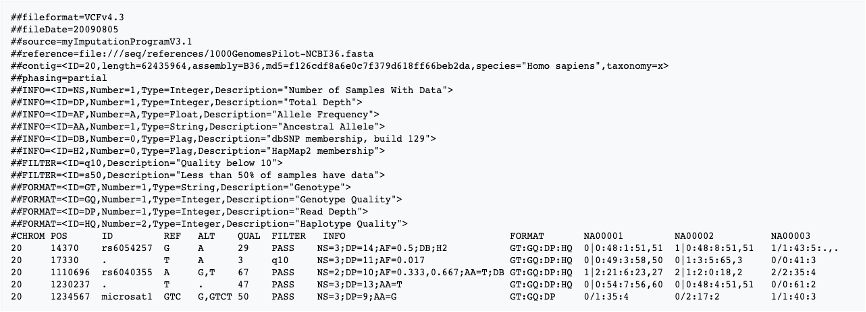
\includegraphics[width=1\columnwidth]{body/image/3-2.png}
    \captionsetup{labelfont=bf}
    \renewcommand{\baselinestretch}{1.0}
    \vspace{-1cm}
    \caption[VCF format]{Example for VCF format.}
    \label{f3-2}
\end{figure}

\begin{figure}[H]
    \centering
    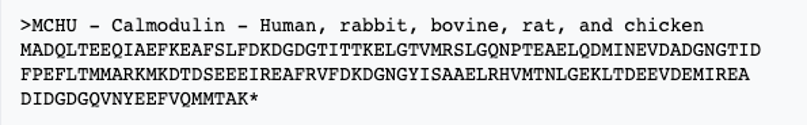
\includegraphics[width=1\columnwidth]{body/image/3-3.png}
    \captionsetup{labelfont=bf}
    \renewcommand{\baselinestretch}{1.0}
    \vspace{-1cm}
    \caption[FASTA format]{Example for FASTA format.}
    \label{f3-3}
\end{figure}

One of the reasons for reference bias is that the reference genome cannot contain individual differences. And our hypothetical sequence is a sequence that combines reference genome and variant, simulate the occur of mutation of the reference sequence by combining variant, make it includes individual differences. So, we will base on the information of each variant in the VCF file, including variant position (POS), chromosome name (CHROM), sequence before mutation (REF), and sequence after mutation (ALT) to generate a hypothetical sequence. 

For each hypothetical sequence, we will according to the variant position, replace sequence before mutation (REF) to sequence after mutation (ALT), at the same time we will extract the reference genome part front and back in this region, and the length will be the length of a read, The length of this area is long enough to include all the reads we are interested in and also include individual differences. Figure  \ref{f3-4} illustrates in detail how we generate a hypothetical sequence based on different types of variants.

We hope to find a read that matches our hypothetical sequence in the FASTQ file to achieve the effect of reducing the reference bias
\vspace{1cm}
\begin{figure}[H]
    \centering
    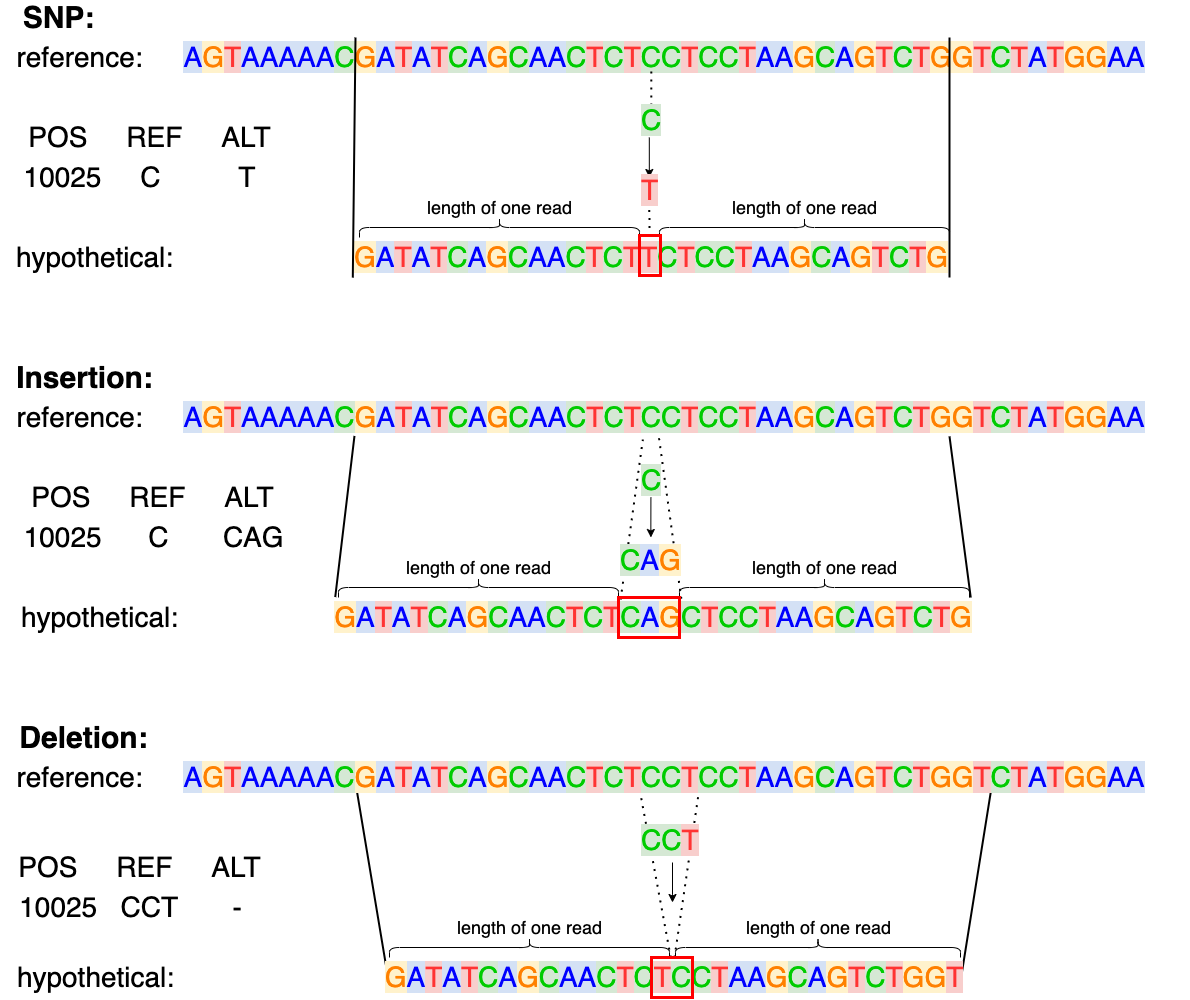
\includegraphics[width=1\columnwidth]{body/image/3-4.png}
    \captionsetup{labelfont=bf}
    \renewcommand{\baselinestretch}{1.0}
    \vspace{-0.5cm}
    \caption[construct hypothetical sequence]{Three different cases to construct hypothetical sequence.}
    \label{f3-4}
\end{figure}

\section{Read-index}

Next is an important step for us to find the read that matches our hypothetical sequence. But if we follow the practice of BWA-MEM, looking for read in FASTQ file will cost us a lot of time. 

First for general practice, hypothetical sequence is the reference genome, and we need to map reads on this, just like alignment. so we need to construct index for each hypothetical sequence and then query all the read in FASTQ file. As we knew that build BWT index need $O(nlogn)$  (n is reference length)to constructed, and query will be $O(m)$ (m is read length)for each read.
\begin{flushleft}
In general situation, Time spent each query as follows: 
\end{flushleft} 
\begin{center}
    $O(m)+O(nlogn)$
\end{center}  

It is indeed a very efficient method in normal times. It only needs to query once for each read, because all reads only need to be aligned to one reference genome sequence. But in our situation, our hypothetical sequence (reference) will not only have one. For each variant we will establish a hypothetical sequence, so if we follow the traditional method, we need to search all the reads every time, our speed will be very slow.

But what if we construct index for read and used our hypothetical sequence to query?
\begin{enumerate}
{
    \item We just need to build index once a time.
    \item For each hypothetical sequence, our query will be very fast.
}
\end{enumerate}

\begin{flushleft}
Let's take an example and some assumptions :
\end{flushleft}

In general situations, we need to create an index for each hypothetical and do a complete read search, it will probably take time:
\begin{center}
    $hypothetical\enspace amount\enspace*\enspace(\enspace index\enspace hypothetical\enspace sequence\enspace+\enspace query\enspace all\enspace reads)$
\end{center}  
\begin{flushleft}
Because the hypothetical sequence is very short compared to all reads, the time of its index can be ignored, then its time will probably be:
\end{flushleft}
\begin{center}
    $hypothetical\enspace amount\enspace*\enspace query\enspace all\enspace reads$
\end{center}  

\begin{flushleft}
And through our way of creating a read index, the time will probably be:
\end{flushleft}
\begin{center}
    $index\enspace all\enspace reads\enspace+\enspace(\enspace hypothetical\enspace amount\enspace*\enspace query\enspace hypothetical\enspace sequence)$
\end{center}  
\begin{flushleft}
Also because the hypothetical sequence is very short, we can ignore its query time, then our time will probably be:
\end{flushleft}
\begin{center}
    $index\enspace all\enspace reads\enspace+\enspace(\enspace hypothetical\enspace amount\enspace quickly\enspace queries)$
\end{center}  

According to the above results, we decided to index our read to generate the read -index, which helps us quickly find the matching read. Before indexing, we need to remove some information in read file to convert FASTQ format to FASTA format. This is very simple like (Table \ref{t3-1}) then we can directly call BWA index function to construct read-index.

\vspace{1cm}
\begin{table}[h]
    \centering
    \caption{The difference between FASTQ and FASTA format}
    \vspace{-0.5cm}
    \begin{tabular}{c}
        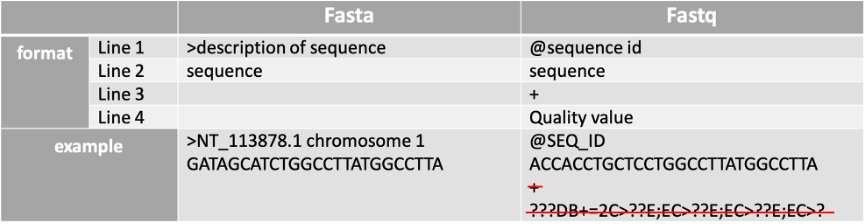
\includegraphics[width=1\textwidth]{body/image/t3-1.png}
    \end{tabular}
    \label{t3-1}
\end{table}

\section{Find Similar Reads}
In previous section, we have introduced how BWA-MEM work, and in this section, we will introduce how do we use BWA and read-index to find the read that matched hypothetical sequence and filter the read we find.

BWA is an open-source software. Fortunately, we can directly use the functions of BWA-MEM and modify part of the code according to EAGLE needs to make it meet our read-index search requirements. Basically, we will use seed alignment based on super maximal exact matching to search for our hypothetical sequence.

The following will describe the changes we made meet to our needs. First of all, for the original BWA-MEM, a read will have only one best matching position, and the others will be marked as secondary (or no primary) (Figure \ref{f3-5}), but for our purposes we simply want to collect all reasonable matches (Figure \ref{f3-6}).

\vspace{1cm}
\begin{figure}[H]
    \centering
    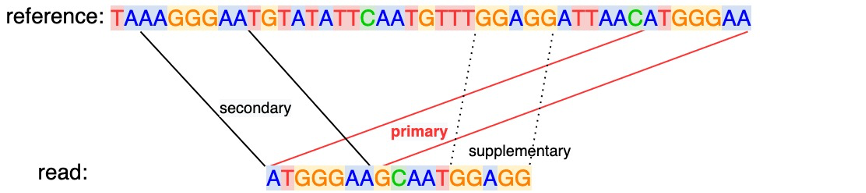
\includegraphics[width=1\columnwidth]{body/image/3-5.png}
    \captionsetup{labelfont=bf}
    \renewcommand{\baselinestretch}{1.0}
    \vspace{-1cm}
    \caption[secondary alignment]{BWA secondary alignment, supplementary alignment.}
    \label{f3-5}
\end{figure}

\vspace{0.5cm}
\begin{figure}[H]
    \centering
    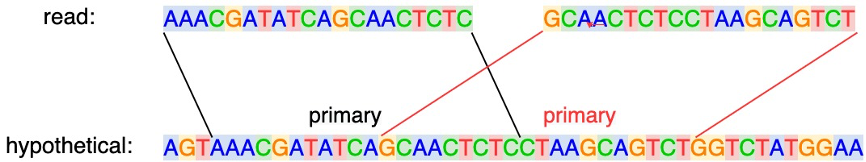
\includegraphics[width=1\columnwidth]{body/image/3-6.png}
    \captionsetup{labelfont=bf}
    \renewcommand{\baselinestretch}{1.0}
    \vspace{-1cm}
    \caption[primary alignment]{The read index is used to find reads matching a hypothetical genome sequence.  BWA marks some matches as primary, etc., but we treat them all the same.}
    \label{f3-6}
\end{figure}

Then we use BWA-MEM to search for our hypothetical sequence using seed alignment based on super maximal exact match, after this, we will get two sets of index as Figure \ref{f3-7} shows, one set represents the start and end positions of the region on the hypothetical sequence, and the other set represents the index of the corresponding read region on the read-index. 

\begin{figure}[H]
    \centering
    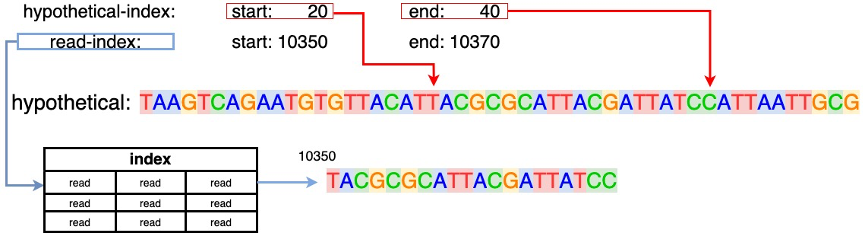
\includegraphics[width=1\columnwidth]{body/image/3-7.png}
    \captionsetup{labelfont=bf}
    \renewcommand{\baselinestretch}{1.0}
    \vspace{-1cm}
    \caption[read-index]{how to find matching read through read-index.}
    \label{f3-7}
\end{figure}

Through the index of hypothetical sequence, we can check whether it contains variant, if not, we will filter it ,like Figure \ref{f3-8} shows. End of this step, we will get a set of meet the requirements read, then we can add to the pileup

\vspace{1cm}
\begin{figure}[H]
    \centering
    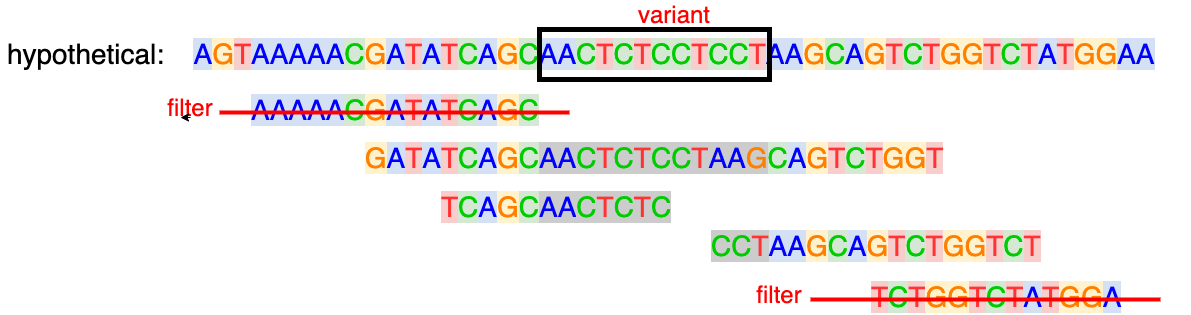
\includegraphics[width=1\columnwidth]{body/image/3-8.png}
    \captionsetup{labelfont=bf}
    \renewcommand{\baselinestretch}{1.0}
    \vspace{-1cm}
    \caption[Filter reads]{Filter reads that didn't overlap variant.}
    \label{f3-8}
\end{figure}

\section{Add reads to the pileup and generate information}
In the last step, we need to compare all the read sets obtained in the previous step with the read in the pileup. What is the pileup? First, in the BAM file, we can observe that the read is mapped to a position on reference genome. Many reads may alignment at the same region, which is called the pileup. Our final goal is to find reads that overlap with the same variant position but do not exist in the pileup, (Figure \ref{f3-9} shows the pileup reads which overlap on a variant position.)

\vspace{1cm}
\begin{figure}[H]
    \centering
    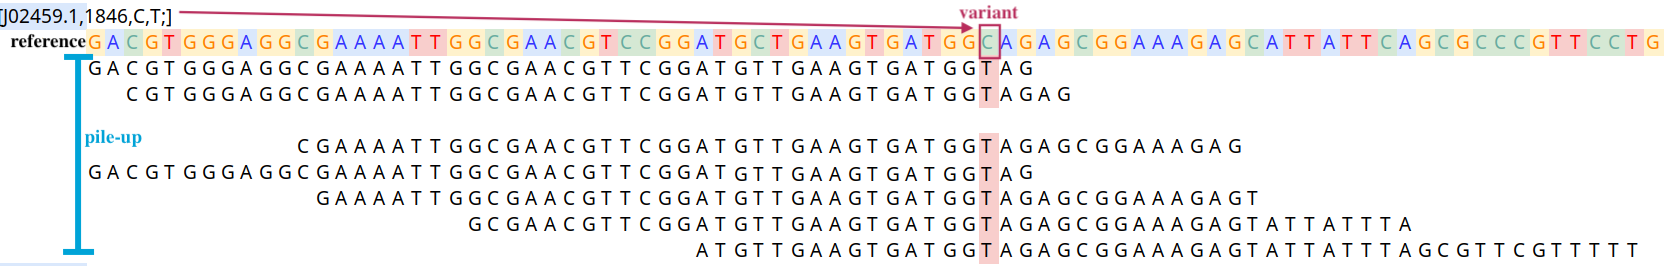
\includegraphics[width=1\columnwidth]{body/image/3-9.png}
    \captionsetup{labelfont=bf}
    \renewcommand{\baselinestretch}{1.0}
    \vspace{-1cm}
    \caption[pileup]{pileup on variant position.}
    \label{f3-9}
\end{figure}

We can get the pileup with BAM file quickly through utility library HTSlib, and after we compare the read set with these pileup reads, if the read does not exist in the pileup, it means that we have got the results we want. So, next step for our work is to convert this read, and use the two sets of index obtained in the previous step to generate some essential information that will be needed in our eagle calculation, like SAM flag and CIGAR string, SAM flag is represents the mapping status of this reads and CIGAR string is alignment console of this read. We will explain how we get CIGAR string through two sets of indexes.

And if we get the SAM flag and CIGAR directly through these two sets of indexes, what we get is the alignment information of hypothetical sequence mapping to read, like previous Figure \ref{f3-8} shows, but what EAGLE needs is the alignment information of read mapping to reference sequence. So we need do some processing on index.

First of all, one of the sets is read index, which represents the position of read in read-index, we can directly obtain our read through it.	Another set is the start and end on our hypothetical sequence, this is what we said before, the corresponding mapping region of read. We need to project this region onto reference genome to help us produce the alignment of read to reference genome.

\begin{flushleft}
This problem can be divided into 4 cases: (Figure 3-10)
\end{flushleft}
\begin{figure}[H]
    \centering
    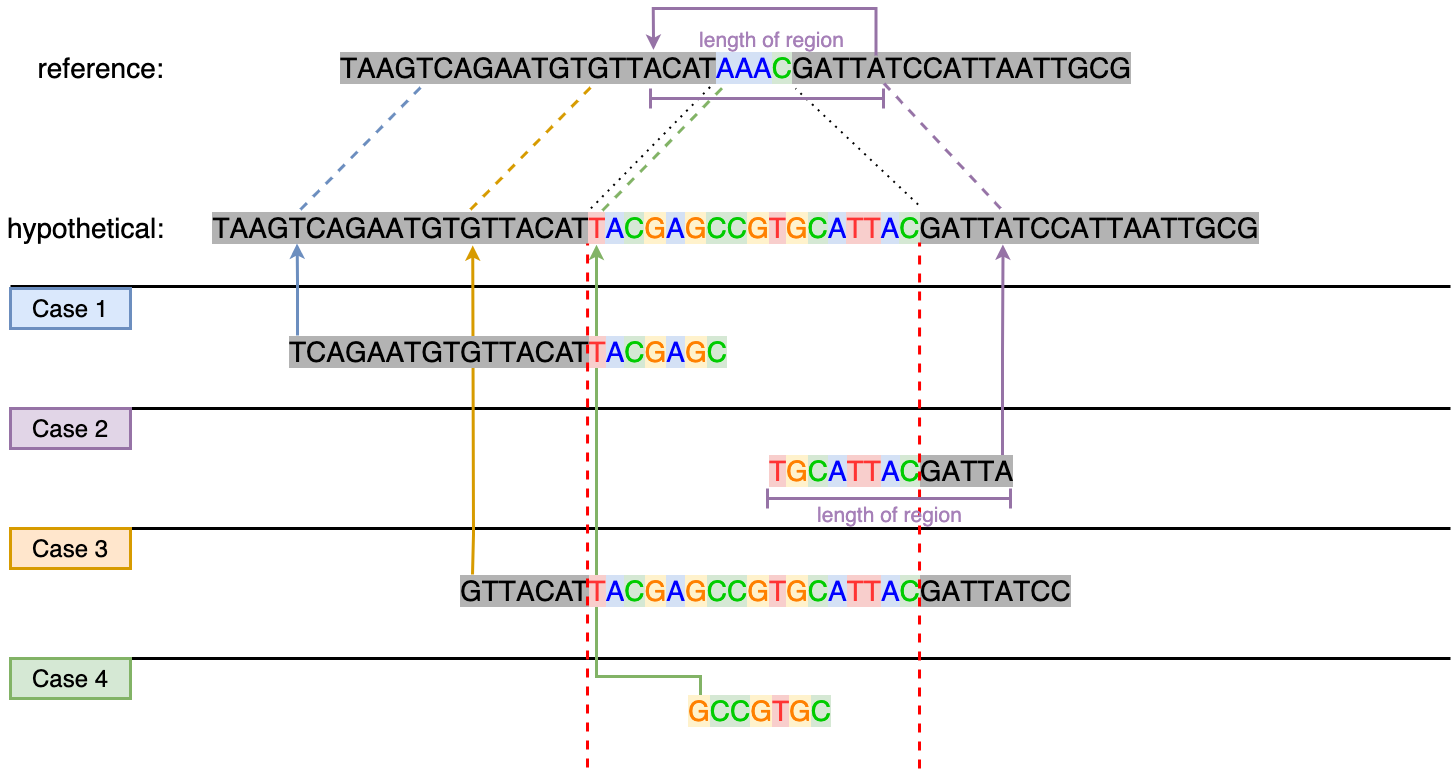
\includegraphics[width=1\columnwidth]{body/image/3-10.png}
    \captionsetup{labelfont=bf}
    \renewcommand{\baselinestretch}{1.0}
    \vspace{-1cm}
    \caption[alignment read]{Four cases related read to variant.  A read may overlap with part of a variant (left or right side), may completely include a variant, or be included by the variant.}
    \label{f3-10}
\end{figure}

\begin{enumerate}
    \item the tail of read sequence overlapped with variant.
    \item the front of read sequence overlapped with variant.
    \item the center of read sequence overlapped with variant
    \item all of read sequence overlapped with variant
\end{enumerate}

For first case and third case we can just directly get the position in reference, and forth case we use the position of variant. A different example is second case, in this case, we need to use the end of the region to push-back the position.

In the last step, we already have read mapping position on reference genome, so that we can create read alignment information. Most of them are nothing special and will not change as we change the alignment position, except for CIGAR string, we need to convert it from hypothetical sequence's alignment information mapped against read to read's alignment information mapped against reference sequences (Figure \ref{f3-11}). we use small function to constructed CIGAR string for our read.

\vspace{1cm}
\begin{figure}[H]
    \centering
    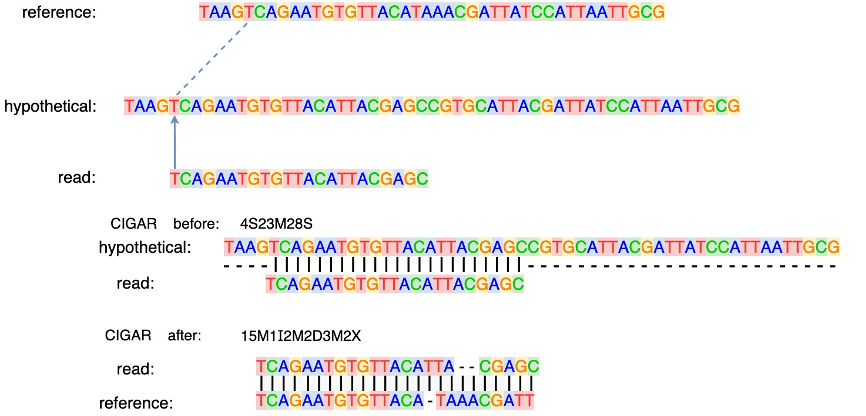
\includegraphics[width=1\columnwidth]{body/image/3-11.png}
    \captionsetup{labelfont=bf}
    \renewcommand{\baselinestretch}{1.0}
    \vspace{-1cm}
    \caption[CIGAR strings]{ how to convert CIGAR strings.}
    \label{f3-11}
\end{figure}

Go through all the steps we can add read to the pileup for eagle to calculate likelihood.




